%-------- Document Class  ------------------------------------------------------------------------------------------------------------------------------------------------
\documentclass[a4paper,11pt]{scrartcl}
\usepackage[margin=1cm
%,showframe% <- only to show the page layout
]{geometry}
\usepackage[utf8]{inputenc}

%-------- Multi-file  ---------------------------------------------------------------------------------------------------------------------------------------------------------
\usepackage{subfiles}

%-------- Preambolo  --------------------------------------------------------------------------------------------------------------------------------------------------
%Per le Figure
\usepackage[english]{babel}
\usepackage{graphicx}

%simboli matematici strani quali unione disgiunta
\usepackage{amssymb}

%Scrivere Sotto i simboli
\usepackage{amsmath}

%Diagrammi Commutativi
\usepackage{tikz}
\usetikzlibrary{matrix}

%Il simbolo di Identità
\usepackage{dsfont}

%Per riflettere i simboli...
\usepackage{graphicx}


%link iNTERNET
\usepackage{hyperref}

%Enumerate with letters
\usepackage{enumerate}

%Slash over letter
\usepackage{cancel}

%Usare bibiliografia bibtex
%\bibliographystyle{plain}

%Danger sign
\usepackage{fourier}

%:=
\usepackage{mathtools}

%http://tex.stackexchange.com/questions/8625/force-figure-placement-in-text
\usepackage{caption}


%subsection numbering
 \setcounter{tocdepth}{3} % if you want all the levels in your table of contents

%Common symbols
%Common math symbols
	%Number fields
		\newcommand{\Real}{\mathbb{R}}
		\newcommand{\Natural}{\mathbb{N}}
		\newcommand{\Relative}{\mathbb{Z}}
		\newcommand{\Rational}{\mathbb{Q}}
		\newcommand{\Complex}{\mathbb{C}}
	
%equality lingo
	%must be equal
		\newcommand{\mbeq}{\overset{!}{=}} 

% function
	%Domain
		\newcommand{\dom}{\mathrm{dom}}
	%Range
		\newcommand{\ran}{\mathrm{ran}}
	

% Set Theory
	% Power set (insieme delle parti
		\newcommand{\PowerSet}{\mathcal{P}}

%Differential Geometry
	% Atlas
		\newcommand{\Atlas}{\mathcal{A}}
	%support
		\newcommand{\supp}{\textrm{supp}}

	
	
%Category Theory
	%Mor set http://ncatlab.org/nlab/show/morphism
%		\newcommand{\hom}{\textrm{hom}}

%Geometric Lagrangian Mechanics
	% Kinematic Configurations
		\newcommand{\Conf}{\mathtt{C}}
	%Solutions Space
		\newcommand{\Sol}{\mathtt{Sol}}
	%Lagrangian class
		\newcommand{\Lag}{\mathsf{Lag}}
	%Lagrangiana
		\newcommand{\Lagrangian}{\mathcal{L}}
	%Data
		\newcommand{\Data}{\mathsf{Data}}
	%unique solution map
		\newcommand{\SolMap}{\mathbf{s}}
	%Classical Observables
		\newcommand{\Obs}{\mathcal{E}}	
	%Phase Space
		\newcommand{\Phase}{\mathcal{M}}	

		\
		
%Peierls (per non sbagliare più)
		\newcommand{\Pei}{Peierls}

%Accented Letters
\usepackage[utf8]{inputenc}

%Temporaneo, Aggiunta della mia classe teorem... Deve diventare un pacchetto!
\input{../Latex-Theorem/TheoremTemplateToninus.tex}
%Common math symbols
	%Number fields
		\newcommand{\Real}{\mathbb{R}}
		\newcommand{\Natural}{\mathbb{N}}
		\newcommand{\Relative}{\mathbb{Z}}
		\newcommand{\Rational}{\mathbb{Q}}
		\newcommand{\Complex}{\mathbb{C}}
	
%equality lingo
	%must be equal
		\newcommand{\mbeq}{\overset{!}{=}} 

% function
	%Domain
		\newcommand{\dom}{\mathrm{dom}}
	%Range
		\newcommand{\ran}{\mathrm{ran}}
	

% Set Theory
	% Power set (insieme delle parti
		\newcommand{\PowerSet}{\mathcal{P}}

%Differential Geometry
	% Atlas
		\newcommand{\Atlas}{\mathcal{A}}
	%support
		\newcommand{\supp}{\textrm{supp}}

	
	
%Category Theory
	%Mor set http://ncatlab.org/nlab/show/morphism
%		\newcommand{\hom}{\textrm{hom}}

%Geometric Lagrangian Mechanics
	% Kinematic Configurations
		\newcommand{\Conf}{\mathtt{C}}
	%Solutions Space
		\newcommand{\Sol}{\mathtt{Sol}}
	%Lagrangian class
		\newcommand{\Lag}{\mathsf{Lag}}
	%Lagrangiana
		\newcommand{\Lagrangian}{\mathcal{L}}
	%Data
		\newcommand{\Data}{\mathsf{Data}}
	%unique solution map
		\newcommand{\SolMap}{\mathbf{s}}
	%Classical Observables
		\newcommand{\Obs}{\mathcal{E}}	
	%Phase Space
		\newcommand{\Phase}{\mathcal{M}}	

		\
		
%Peierls (per non sbagliare più)
		\newcommand{\Pei}{Peierls}	%Common symbols
\usepackage{glossaries}

\makenoidxglossaries

%How to:
%affinchè la voce venga printata nella lista va prima chiamata nel testo come e.g. \gls{Bundle}
%ricordarsi di chiamarlo almeno una volta così, dopo usare il command per evitare il ripetuto hyperref
% anche se si potrebbe evitare visto che il quadratino del link non dovrebbe apparire in stampa

%Advanced Differential Geometry
\newglossaryentry{Bundle}%
{%
	name={\ensuremath{E = (E,\pi , M;Q)}},
	description={ Fiber Bundles $\pi: E\rightarrow M$ with typical fiber $Q$},
    sort={B}
}

\newglossaryentry{Sections}%
{%
	name={\ensuremath{\Gamma^\infty(E)}},
	description={ Smooth sections on the bundle $E$.},
    sort={S}
}


%Geometric Lagrangian Mechanics
	% Kinematic Configurations
	\newglossaryentry{Conf}%
	{%
		name={\ensuremath{\Conf}},
		description={ Kinematic Configurations set}
	}

	%Solutions Space
	\newglossaryentry{Sol}%
	{%
		name={\ensuremath{\Sol}},
		description={ Dynamic Configurations set}
	}

		
	%Lagrangian class
		\newglossaryentry{Lag}%
	{%
		name={\ensuremath{\Lag}},
		description={ Set of Lagrangian densities.}
	}
		
	%Lagrangiana
	\newglossaryentry{Lagrangian}%
	{%
		name={\ensuremath{\Lagrangian}},
		description={ Lagriangian density of the system.}
	}
		
	%Data
	\newglossaryentry{Data}%
	{%
		name={\ensuremath{\Data}},
		description={ Inital Data set.}
	}
		
	%unique solution map
	\newglossaryentry{SolMap}%
	{%
		name={\ensuremath{\SolMap}},
		description={ Map that map a fixed initial data to the unique solution.}
	}
		
	%Classical Observables
	\newglossaryentry{Obs}%
	{%
		name={\ensuremath{\Obs}},
		description={ Set of all classical observables.}
	}

	%Phase Space
	%Classical Observables
	\newglossaryentry{Phase}%
	{%
		name={\ensuremath{\Phase}},
		description={ Phase space.}
	}



\hyphenation{gua-ran-te-ed}
\hyphenation{Ha-da-mard}
\hyphenation{Rieman-nian}
\pagestyle{empty}

%Temporaneo, Aggiunta della mia classe teorem... Deve diventare un pacchetto!
\input{../../Latex-Theorem/TheoremTemplateToninus.tex}

%---------------------------------------------------------------------------------------------------------------------------------------------------------------------
\title{Demystification of Peierels Brackets construction}
\author{Antonio Michele Miti}
\date{\vspace{-5ex}} % workaround to omit the Date !

%\/\/\/\/\/\/\/\/\/\/\/\/\/\/\/\/\/\/\/\/\/\/\/\/\/\/\/\/\/\/\/\/\/\/\/\/\/\/\/\/\/\/\/\/\/\/\/\/\/\/\/\/\/\/\/\/\/\/\/\/\/\/\/\/\/\/\/\/\/
\begin{document} %\/\/\/\/\/\/\/\/\/\/\/\/\/\/\/\/\/\/\/\/\/\/\/\/\/\/\/\/\/\/\/\/\/\/\/\/\/\/\/\/\/\/\/\/\/\/\/\/\/\/\/\/\/\/\/\/\/\/\/

	%\maketitle
	\section*{Demystification of Peierels Brackets construction}

	%Abstact dynamical system
	\begin{definition}[(Abstract) Dynamical System]\label{Def:AbstracDynamicalSystem}
		Pair $(E,P )$ composed of:
		\begin{compactitemize}
			\item $E \xrightarrow{\pi} M \qquad $ \emph{"configuration bundle"}\\
			smooth fiber bundle of typical fiber $Q$ on  manifold $M$.
			\item	$ P : \Gamma^\infty(E) \rightarrow \Gamma^\infty(E) \qquad $  \emph{"(Dynamics) motion operator"}\\
			differential operator in the sense that it is represented by a linear combination of partial derivative in every local chart.
		\end{compactitemize}
	\end{definition}

		\begin{minipage}{0.5\textwidth}
			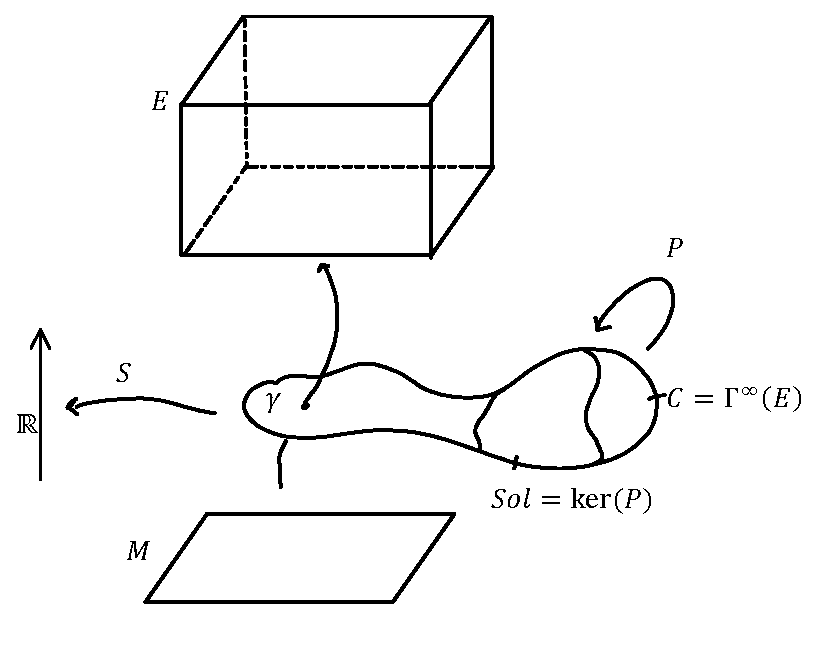
\includegraphics[width=\textwidth]{../Pictures/AbstractFieldTheory}
		\end{minipage}
		\begin{minipage}{0.5\textwidth}
			\begin{definition}[Space of kinematics (off-shell) configurations]
				\begin{displaymath}
					\Conf \coloneqq \Gamma^\infty(M,E)
				\end{displaymath}
			\end{definition}
			\begin{definition}[Space of Dynamics (on-shell) configurations]\label{Def:SolSpace}
				The subset of $\Conf$ containing all the smooth solutions of the motion equations corresponding to the  dynamical operator 
				$P: \Conf \rightarrow \Conf$.
				\begin{displaymath}
					\gls{Sol} \coloneqq \ker(P) = \left\{\left. \gamma \in \Conf \quad\right\vert  R(P)\left(f\right) = 0 \quad \forall \textrm{\tiny local chart representation}\right\}
				\end{displaymath}
				where we have denoted respectively as $R(P)$ and $f$ the local chart representation of $P$ and $\gamma$ on the same chart.
			\end{definition}
		\end{minipage}



	% Abstract Lagrangean system
	\begin{definition}[Lagrangian System ( of $r$-th order)]
		The pair $(E, \mathcal{L} )$ composed of:
		\begin{compactitemize}
			\item $E \xrightarrow{\pi} M \qquad$ \emph{"configuration bundle"}\\
			smooth fiber bundle of typical fiber $Q$ on the oriented pseudo-Riemannian manifold $(M,g,\mathfrak{o})$.
			\item	$ \gls{Lagrangian} : J^r E \rightarrow \wedge^m T^*M \qquad$ \emph{"Lagrangian (Density)" of r-th order}\\
			bundle-morphism from the r-th Jet Bundle to  the top-dimensional forms bundle over the base manifold $M$.
		\end{compactitemize}
	\end{definition}

	\begin{definition}[Lagrangian Densities on the bundle $E$ (of $r-$th order) ]\label{Def:LagrangianDensities}
		Elements of th set:
		\begin{displaymath}
			\Lag^r (E) \coloneqq \Gamma^\infty \left( \Hom\biggr(J^r E,\quad \bigwedge^m( T^*M)\biggr) \right) \cong \big\{f:\Gamma^\infty(J^r E) \rightarrow \Omega^m(M)  \big\}
		\end{displaymath}
		where $\Omega^m(M)$ is the common name for $\Gamma^\infty \big( \bigwedge^m( T^*M) \big)$ in the context of Grassmann algebras.
		\footnote{	The equivalence states the fact that a bundle-morphism induces a map between the sections.}
	\end{definition}
	%this choice fix the "Dynamical identity" of the considered system. (Correzione CD)
	\begin{proposition}
		$\Lag^r(E)$ has an vector space structure inherited by the linear structure of $\Omega(M)$.
	\end{proposition}

	\begin{definition}[Lagrangian functional]\label{Def:LagrangianFunctionals}
		The map :
		\begin{displaymath}
			\mathcal{O}_\Lagrangian : \Conf \rightarrow D'(M)
		\end{displaymath}
		(where  $D'(M)$ is the space of regular distribution over $M$)\\
		whose action on any configuration\footnote{Recalling the correspondence form differentiable sections to jet it is possible to see the Lagrangian as acting directly on $\Conf$.} 
		$\phi \in \Conf$, evaluated on the test-function $f \in C^\infty_0(M)$, it is given by:
		\begin{displaymath}
			\mathcal{O}_\Lagrangian [\phi] (f) = \int_M \Lagrangian [\phi] f \textrm{d}\mu
		\end{displaymath}
		where $d\mu = d\textrm{Vol}_\mu$ is the volume form induced by the metric and the orientation on $M$
	\end{definition}

	\begin{definition}[Euler-Lagrange operator (relative to the Lagrangian density $\chi \in \Lag^1(E)$)]
		The  differential operator $Q_\chi : \Conf \rightarrow \Conf$	, such that:
		\begin{displaymath}
			Q_\chi (\gamma) = \Biggr( \nabla_\mu \biggr( \frac{\partial \chi}{\partial(\partial_\mu \phi)} \biggr\vert_\gamma \biggr) - \frac{\partial \chi}{\partial \phi}\biggr\vert_\gamma \Biggr) \qquad \forall \gamma \in \Conf	
		\end{displaymath}
		Where $\nabla_\mu$ is the covariant derivative corresponding to the background metric $g$.
		\footnote{$\frac{\partial \chi}{\partial(\partial_\mu \phi)}$ has the be intended as the Lagrangian density constructed differentiating $\chi(\phi, \partial_\mu)$ as an ordinary function, treating its functional entries as an usual scalar variable.}
	\end{definition}

	\subsection*{Peirels Constuction}

	\begin{definition}[Disturbance]
		By \emph{"disturbance"} we mean a time-compact supported Lagrangian density $\chi \in \Lag$,\\
		I.e. the top form $\chi(\phi)$ is time-compact supported for all $\phi \in \Conf$.
	\end{definition}

	\begin{remark}
	 Disturbance is usually seen as a perturbation on the Lagrangian of the system:
		\begin{displaymath}
			\Lagrangian \rightsquigarrow \Lagrangian' = \Lagrangian + \epsilon\cdot \chi
		\end{displaymath}
		where $\epsilon$  is a real modulation parameter.\\
		Since $\Lag$ is linear we have that $\Lagrangian'$ is still a suitable Lagrangian of the system.	
	\end{remark}

	\begin{definition}[Jacobi Equation ( relative to a disturbance $\chi$)]
		Is the operator equation
		\begin{equation}\label{PeierlJacobiEqLin}
			P \eta = - Q_\chi \phi(x)
		\end{equation}
		where $\phi \in \Sol$ is a fixed solution of the unperturbed motion and $\eta \in \Conf$.
	\end{definition}
	
	\begin{proposition}
		To find a solution of the Jacobi equations is equivalent to find the solution of 
   			\begin{displaymath}
   			   	\begin{cases} 
  					& P_\epsilon \phi'(x) = (P + \epsilon Q_\chi ) \phi'(x) = o(\epsilon)  \\ 
					& P \phi(x) = 0 \\
					& \phi' = \phi + \epsilon \eta
				\end{cases} 			
   			\end{displaymath}		
		i.e. the solutions of the disturbed (by a disturbance $\chi$) Motion equation obtainable by a small perturbation of $\Sol$ moduled by the fixed disturbance $chi$
	\end{proposition}	
	Let be $B:\Conf \rightarrow D'(M)$ a differentiable functional \footnote{The precise notion of continuity require the specification of a (infinite dimensional) manifold structure on $\Conf$.}
	\begin{definition}[Effect Operator ( of a disturbance $\chi$ on B )]
		The map
		$$\EffectOp : C^1(\Conf,D'(M)) \rightarrow C^0(\Sol,D'(M))$$
		such that:
		$$	\EffectOp_\chi^\pm B ( \phi_0) \coloneqq \lim_{\epsilon \rightarrow 0} \biggr( \frac{B(\phi_\epsilon^\pm) - B (\phi_0)}{\epsilon} \biggr)  \qquad \forall \phi_0 \in \Sol $$
	\end{definition}
	\begin{definition}[Peierls Bracket]
 		The binary operator
		$$ \{\cdot,\cdot\}:\Lag_{\textrm{tc}} \times \Lag_{\textrm{tc}} \rightarrow \Real 	$$
		such that:
		$$ \{\chi, \omega \}(\phi_0) \coloneqq \EffectOp_\chi^- \mathcal{O}_\omega (\phi_0) - \EffectOp_\chi^+ \mathcal{O}_\omega(\phi_0) $$
	\end{definition}
	
	
	\subsection*{Symplectic space of field-theoretic systems.}
	Let be:
	\begin{compactitemize}
		\item $\pi : E \rightarrow M $ Vector Bundle on spacetime $M$
		\item $M$  globally hyperbolic
		\item $P= Q_\Lagrangian$ green hyperbolic
	\end{compactitemize}
	
	\begin{definition}[Pairing between two configurations]
		The bilinear mapping:
   			$$ (X,Y) = \int_M <X,Y>_x d\mu(x) $$
			where $d\mu = d\textrm{Vol}_\mu$ is the volume form induced by the metric and the orientation on $M$ and $<\cdot,\cdot>_x$ is bundle inner product on $E$.
			\footnote{The definition is well posed only on 
			$ \dom\big( (\cdot, \cdot) \big) =
			 \big\{(X,Y) \in \Gamma^\infty(E) \times \Gamma^\infty(E) \; 
			 \big\vert \,  <X,Y>_x \in L^1(M,\mu)\big \}$}
	\end{definition}
	Let be $<\cdot,\cdot>_x$ a suitable choice of bundle inner-product such that $P$ results formally self-adjoint.
	\begin{definition}[Pre-Observables (\emph{"off-shell"} )]
		\begin{displaymath}
			\Obs_0 \coloneqq \biggr\{ F_f (\cdot) = ( f, \cdot ) \quad
			\left\vert\quad  f \in \Gamma_0^\infty(E) \right.	\biggr\} \subset \Conf^* 
		\end{displaymath}
		where $\Conf^* $ is the space of continous functional  from $\Conf$ to $\Real$.
	\end{definition}
	
	\begin{proposition}
		The linear map	 $$ F: \Gamma_0^\infty \rightarrow \Obs_0 $$
		which associates to any section $f\in \Gamma_0^\infty(E)$ the associated linear functional,\\ is one-to one and satisfies the separability condition
				$$ \forall \phi, \psi \in \Conf \quad \exists f \in \Gamma_0 \quad \textrm{s.t.} \quad F_f(\phi) \neq F_f(\psi)$$
	\end{proposition}
		\begin{proposition}
		The linear map	 $$ F^\Sol = r^\Sol \circ F : \Gamma_0^\infty \rightarrow \Sol^* $$
		which associates to any section $f\in \Gamma_0^\infty(E)$ the associated linear functional with domain restricted to $\Sol$,\\
		 is not injective
				$$ \ker(F^\Sol) = \frac{\Gamma_0}{P \Gamma_0}$$
	\end{proposition}
	
	\begin{definition}[Classical Observables (\emph{"on-shell"})]
		Is the subset of continuous linear functional on $\Sol$, range of the map $F$:
		$$ \Obs = F \left( \frac{\Gamma_0}{P \Gamma_0} \right) \subset \Sol^*$$
		Such that 
		$$   F_{[f]} (\phi) = F_f(\phi) \qquad \forall \phi \in \Sol ,\; \forall f \in [f] \in \Gamma_0 / P \Gamma_0 $$
		\footnote{This expression is independent from the choice of the representative only on $\Sol$.}
	\end{definition}
	\begin{proposition}
	The mapping
	$$ F: frac{\Gamma_0}{P \Gamma_0} \rightarrow \Obs $$ in one-to-one. So:
	$$ \Obs \simeq frac{\Gamma_0}{P \Gamma_0}$$
	\end{proposition}
	
	\begin{definition}[Field-Theoretic (PreQuantum) Symplectic Space]
		The Pair $(\Obs, \tau)$, where
		$$ \tau\left( [\phi] , [\psi] \right) = (\phi, E \psi) \qquad \forall [f], [g] \in \Obs $$
		is a well-defined (independent from the choice of the representative) symplectic form,
		and $E$ is the unique \emph{Advanced minus Retarded} operator associated to GH operator $P$.
	\end{definition}
	\begin{theorem}
		$\tau$ corresponds to the restriction of the Peierls brackets to the subspace of Lagrangians
		$$\left\{\left. \Lagrangian_\phi \big[\cdot \big] ( x ) = <\phi, \cdot>_x \quad \right\vert  \quad
		\phi \in \Gamma_0^\infty \right\} \subset \Lag^1(E)$$
	\end{theorem}

\end{document} %\/\/\/\/\/\/\/\/\/\/\/\/\/\/\/\/\/\/\/\/\/\/\/\/\/\/\/\/\/\/\/\/\/\/\/\/\/\/\/\/\/\/\/\/\/\/\/\/\/\/\/\/\/\/\/\/\/\/\/\
%\/\/\/\/\/\/\/\/\/\/\/\/\/\/\/\/\/\/\/\/\/\/\/\/\/\/\/\/\/\/\/\/\/\/\/\/\/\/\/\/\/\/\/\/\/\/\/\/\/\/\/\/\/\/\/\/\/\/\/\/\/\/\/\/\/\/\/\/\/
